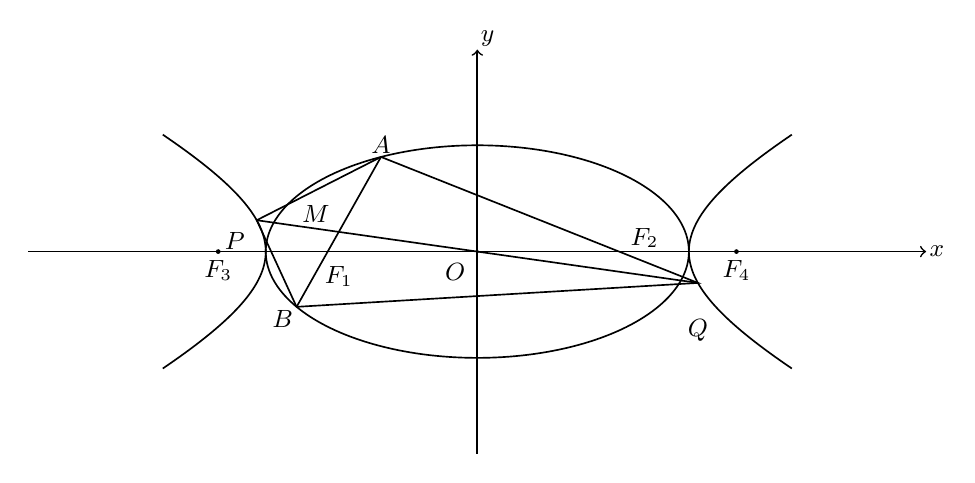
\begin{tikzpicture}[x=1.9cm,y=1.35cm,line width=.6pt]
\tikzset{lbl/.style={font=\small,inner sep=1pt,text opacity=1}}
% curves from exact formulas: ellipse x^2/2+y^2=1, hyperbola x^2/2-y^2=1
\draw[domain=0:360,samples=200,variable=\t] plot ({1.41421356*cos(\t)},{sin(\t)});
\draw[domain=-1.1:1.1,samples=80,variable=\t] plot ({sqrt(2*(1+\t*\t))},\t);
\draw[domain=-1.1:1.1,samples=80,variable=\t] plot ({-sqrt(2*(1+\t*\t))},\t);
% axes
\draw[->] (-3,0) -- (3,0) node[lbl,right] {$x$};
\draw[->] (0,-1.9) -- (0,1.9) node[lbl,above right] {$y$};
% points (A,B on ellipse; P,Q on hyperbola, verified in construction script)
\coordinate (A) at (-0.6438602553,0.8903493617);
\coordinate (B) at (-1.2079915965,-0.5199789913);
\coordinate (P) at (-1.4744195615,0.2948839123);
\coordinate (Q) at (1.4744195615,-0.2948839123);
\coordinate (F1) at (-1,0);
\coordinate (F2) at (1,0);
\coordinate (F3) at (-1.732051,0);
\coordinate (F4) at (1.732051,0);
\coordinate (O) at (0,0);
\coordinate (M) at (-0.9259259259,0.1851851852);
\fill (F3) circle (0.03cm);
\fill (F4) circle (0.03cm);
\fill (O) circle (0.025cm);
% quadrilateral APBQ + diagonals AB and PQ
\draw (A) -- (P) -- (B) -- (Q) -- cycle;
\draw (A) -- (B);
\draw (P) -- (Q);

% labels
\node[lbl,above] at (A) {$A$};
\node[lbl,below left] at (B) {$B$};
\node[lbl,below left=3pt] at (P) {$P$};
\node[lbl,below=12pt] at (Q) {$Q$};
\node[lbl,below=4pt,xshift=4pt] at (F1) {$F_{1}$};
\node[lbl,above right] at (F2) {$F_{2}$};
\node[lbl,below=2pt] at (F3) {$F_{3}$};
\node[lbl,below=2pt] at (F4) {$F_{4}$};
\node[lbl,below left=3pt] at (O) {$O$};
\node[lbl,above left=2pt] at (M) {$M$};
\end{tikzpicture}
